%!TEX root = main.tex
\chapter{Supplementary Results on Camera Calibration Estimation}     % numérotée
\label{annex4}

\DeclareGraphicsExtensions{.pdf,.jpeg,.png,.jpg}
\graphicspath{{annex4_figures/}}

The purpose of this annex is to extend the explanations, results and
analysis presented in the main paper. More results on sun position
estimation, camera parameter estimation and virtual object insertion on
both the SUN360 and HDR dataset are provided. Furthermore, supplementary
explanations on the HDR capture is given.

All the provided examples (images and panoramas) are taken from our test
set, which the neural network has never seen during training nor
validation.

\hypertarget{table-of-contents}{%
\subsection{Table of Contents}\label{table-of-contents}}

\begin{enumerate}
\tightlist
\item
  \protect\hyperlink{sunpos}{Sun Position (extends fig. 6)}
\item
  \protect\hyperlink{virtualobjectinsert}{Virtual Object Insertion
  (extends fig. 9)}
\item
  \protect\hyperlink{camparameval}{Camera Parameters Estimation}

  \begin{enumerate}
  \tightlist
  \item
    \protect\hyperlink{camparamestimperf}{Parameter Estimation
    Performance}
  \item
    \protect\hyperlink{camparaminsertionex}{Object Insertion Examples
    (extends fig. 10)}
  \end{enumerate}
\item
  \protect\hyperlink{HDRcaptures}{HDR Captures (extends sec. 6.3)}
\item
  \protect\hyperlink{virtualobjectinsertHDR}{HDR Virtual Object
  Insertion (extends fig. 11)}
\end{enumerate}

\protect\hypertarget{sunpos}{}{}

\hypertarget{sun-position-estimation}{%
\section{Sun position estimation}\label{sun-position-estimation}}

In this section, we present some additional sun position estimations,
extending the results shown in fig. 6.


\def\mywidth{0.9\linewidth}

\begin{multicols}{2}

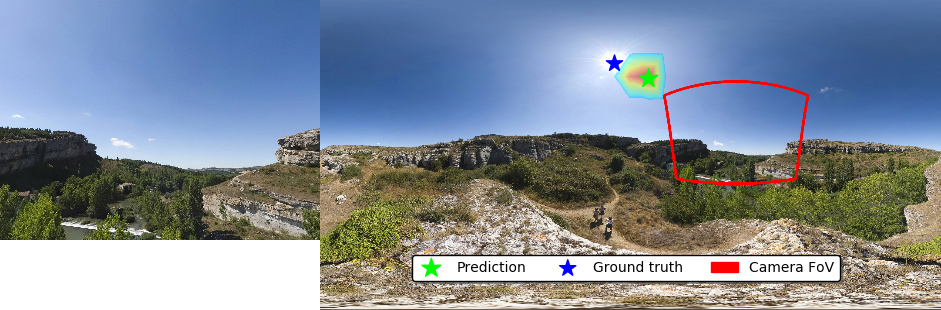
\includegraphics[width=\mywidth]{pano_aacuaoohjiliba_002.jpg}\\
Angular distance: 15.6 degrees

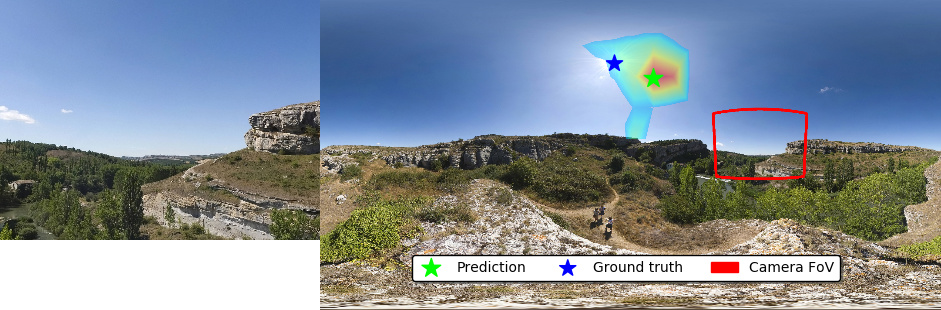
\includegraphics[width=\mywidth]{pano_aacuaoohjiliba_006.jpg}\\
Angular distance: 17.0 degrees

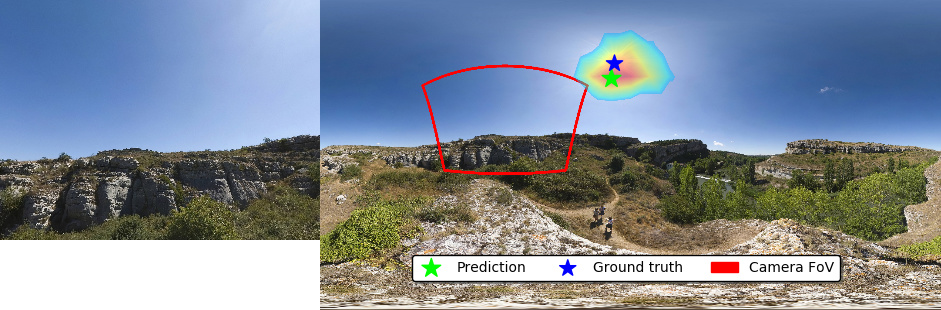
\includegraphics[width=\mywidth]{pano_aacuaoohjiliba_005.jpg}\\
Angular distance: 8.6 degrees

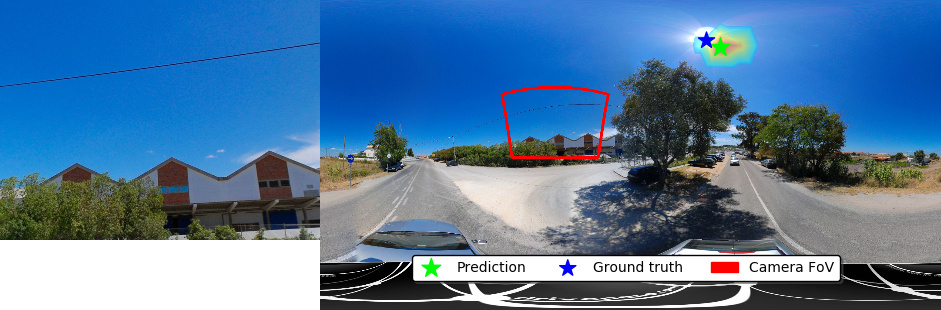
\includegraphics[width=\mywidth]{pano_aaezuadrpeomdf.jpg}\\
Angular distance: 5.4 degrees

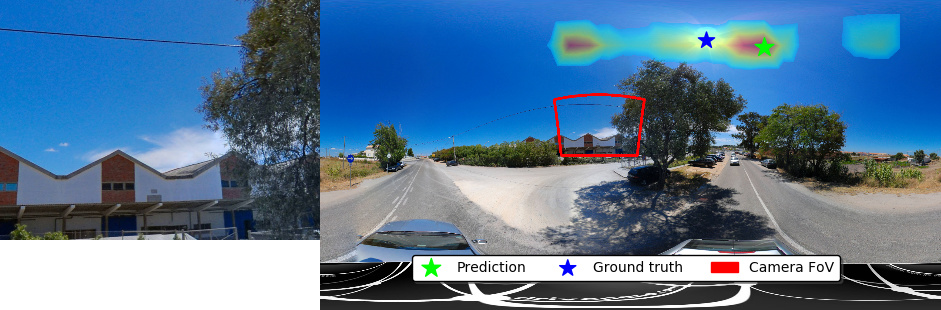
\includegraphics[width=\mywidth]{pano_aaezuadrpeomdf_002.jpg}\\
Angular distance: 14.5 degrees

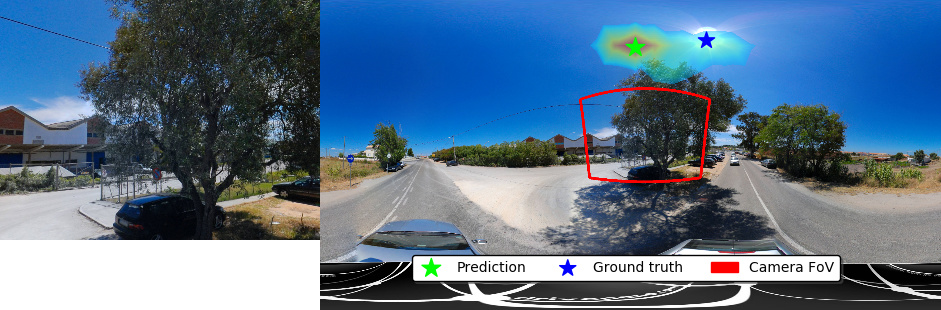
\includegraphics[width=\mywidth]{pano_aaezuadrpeomdf_004.jpg}\\
Angular distance: 17.5 degrees

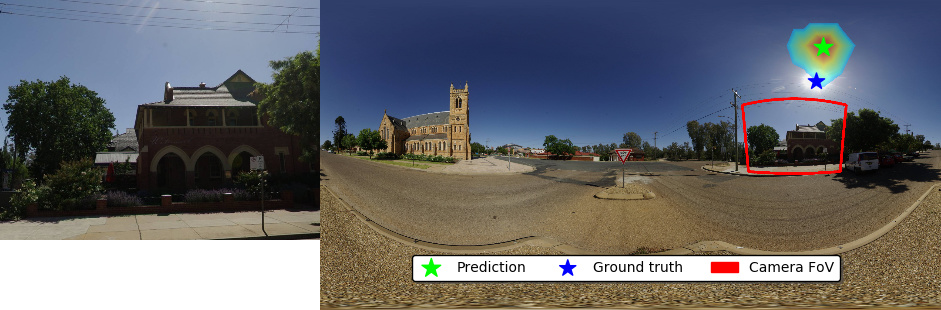
\includegraphics[width=\mywidth]{pano_aagpbpdmorbfwq_005.jpg}\\
Angular distance: 20.1 degrees

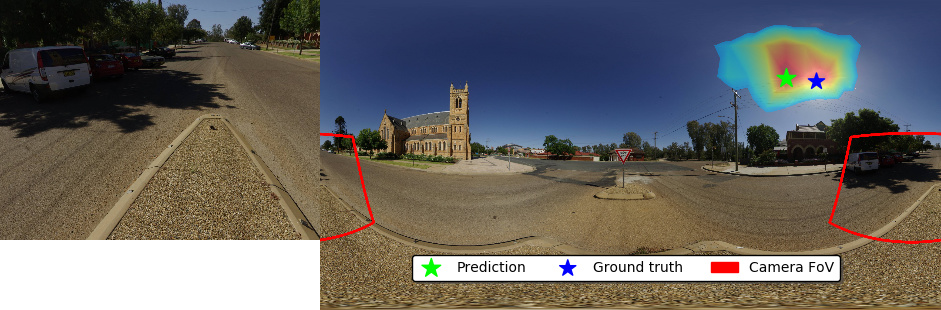
\includegraphics[width=\mywidth]{pano_aagpbpdmorbfwq_006.jpg}\\
Angular distance: 12.8 degrees

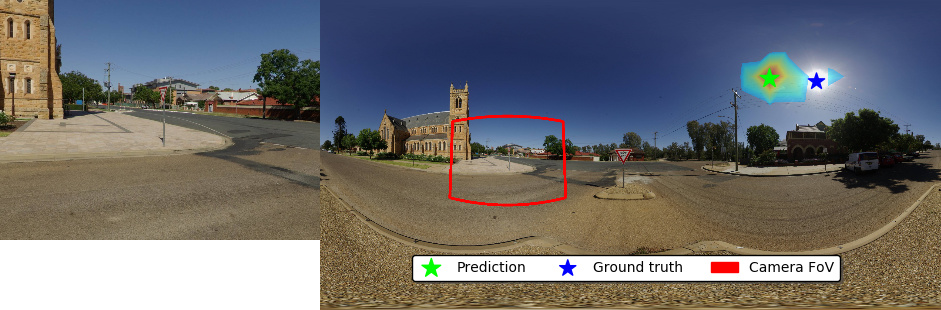
\includegraphics[width=\mywidth]{pano_aagpbpdmorbfwq_002.jpg}\\
Angular distance: 19.5 degrees

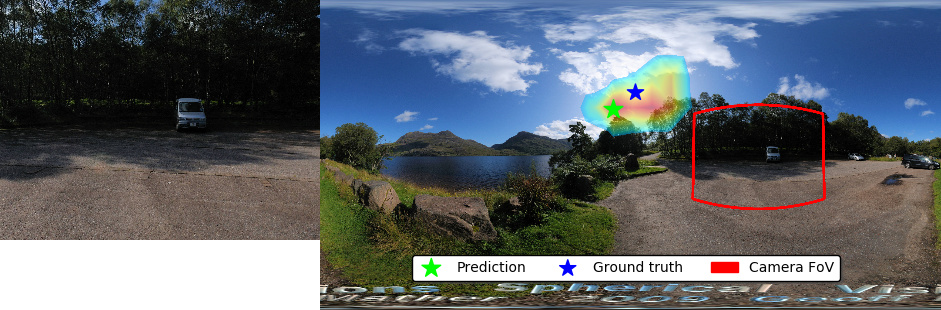
\includegraphics[width=\mywidth]{pano_aaihqlchfeptuj_003.jpg}\\
Angular distance: 14.8 degrees

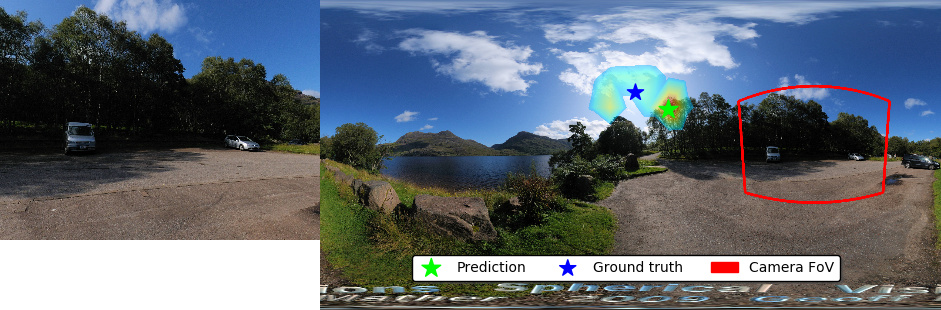
\includegraphics[width=\mywidth]{pano_aaihqlchfeptuj_004.jpg}\\
Angular distance: 18.9 degrees

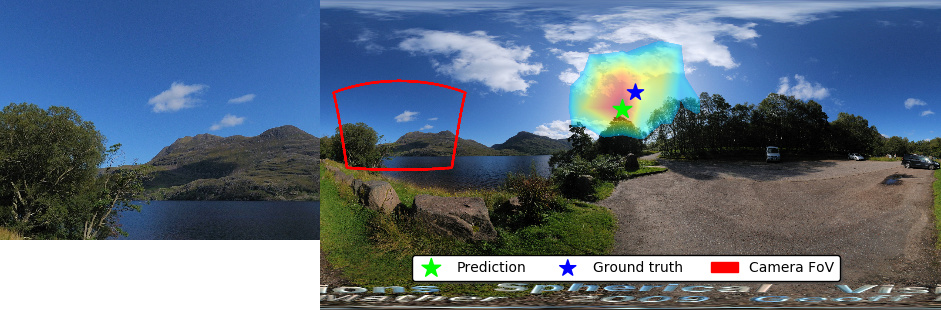
\includegraphics[width=\mywidth]{pano_aaihqlchfeptuj.jpg}\\
Angular distance: 11.8 degrees

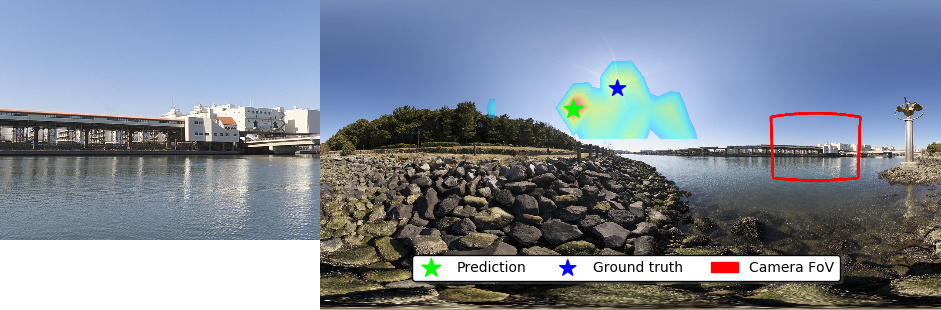
\includegraphics[width=\mywidth]{pano_aakgxuckdrzzpz.jpg}\\
Angular distance: 24.4 degrees

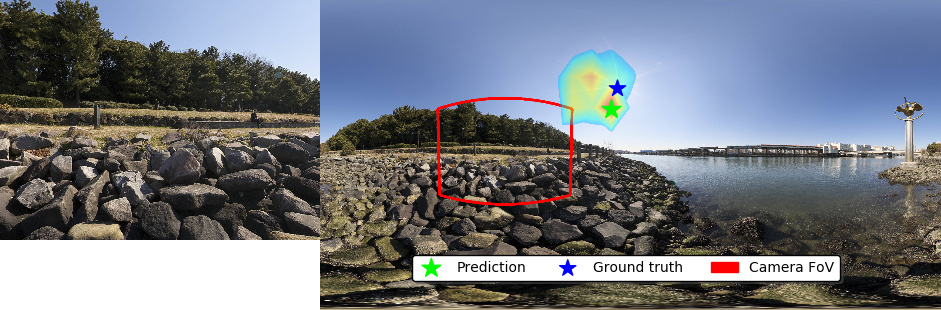
\includegraphics[width=\mywidth]{pano_aakgxuckdrzzpz_003.jpg}\\
Angular distance: 12.4 degrees

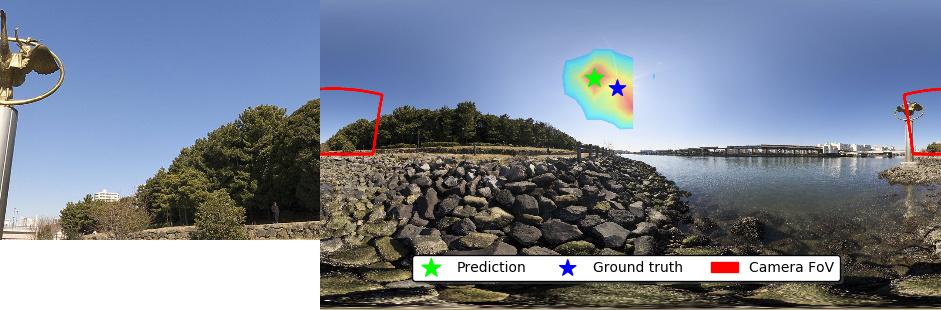
\includegraphics[width=\mywidth]{pano_aakgxuckdrzzpz_002.jpg}\\
Angular distance: 11.3 degrees

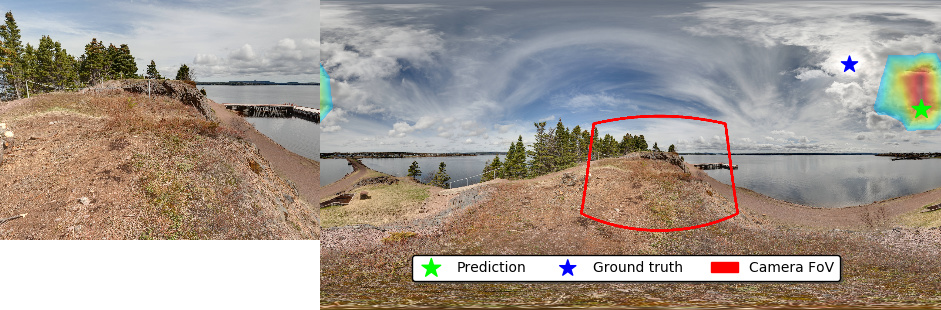
\includegraphics[width=\mywidth]{pano_aakkizvmfscmlr.jpg}\\
Angular distance: 40.4 degrees

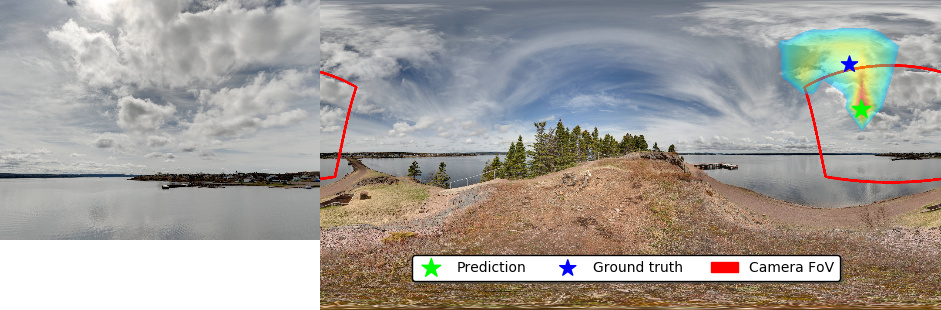
\includegraphics[width=\mywidth]{pano_aakkizvmfscmlr_005.jpg}\\
Angular distance: 26.5 degrees

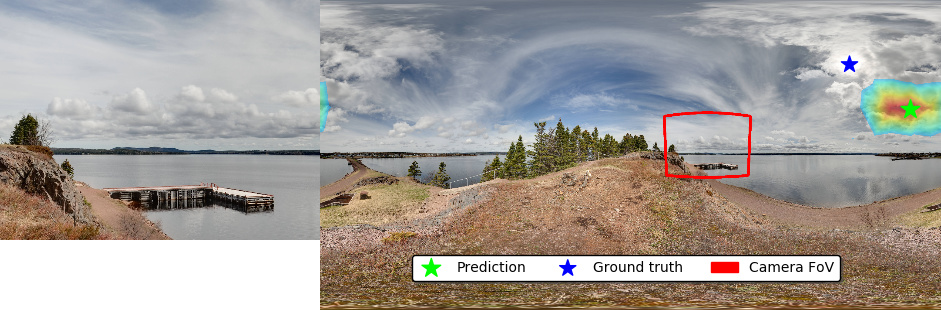
\includegraphics[width=\mywidth]{pano_aakkizvmfscmlr_004.jpg}\\
Angular distance: 37.2 degrees

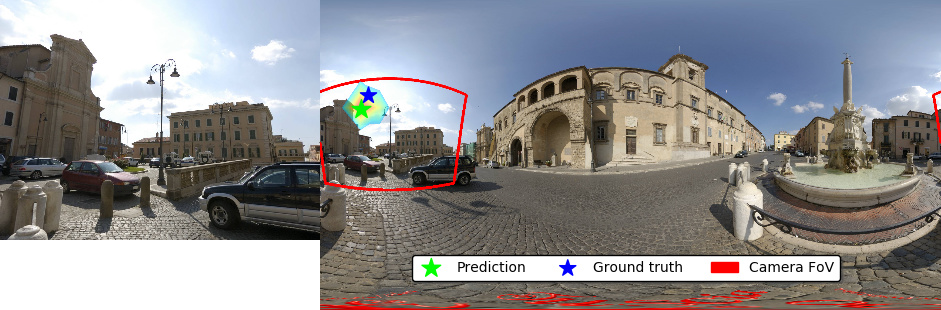
\includegraphics[width=\mywidth]{pano_aakpbaojeqowkb_006.jpg}\\
Angular distance: 8.9 degrees

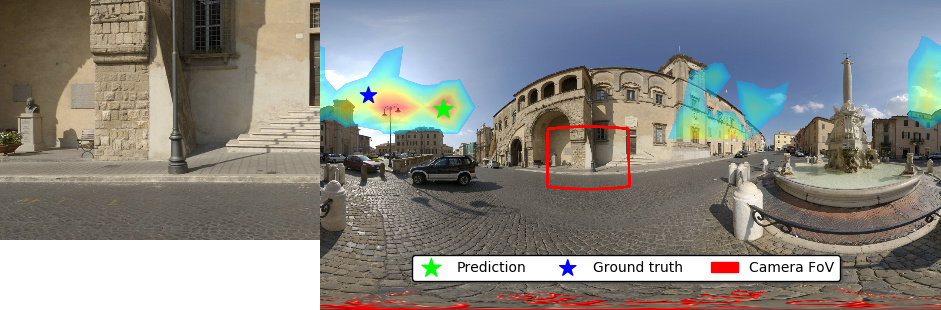
\includegraphics[width=\mywidth]{pano_aakpbaojeqowkb_004.jpg}\\
Angular distance: 37.5 degrees

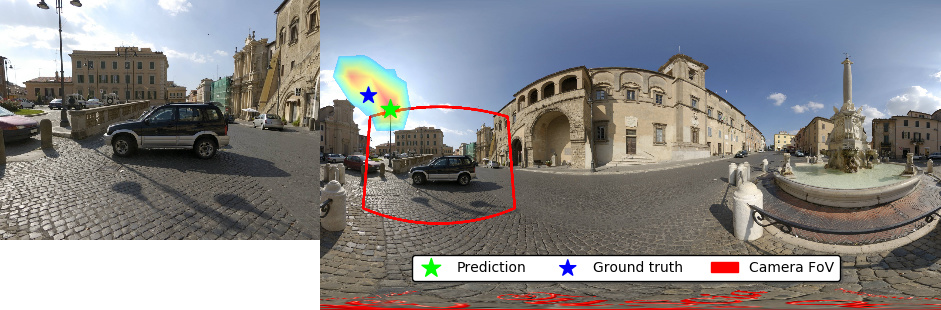
\includegraphics[width=\mywidth]{pano_aakpbaojeqowkb_003.jpg}\\
Angular distance: 13.5 degrees

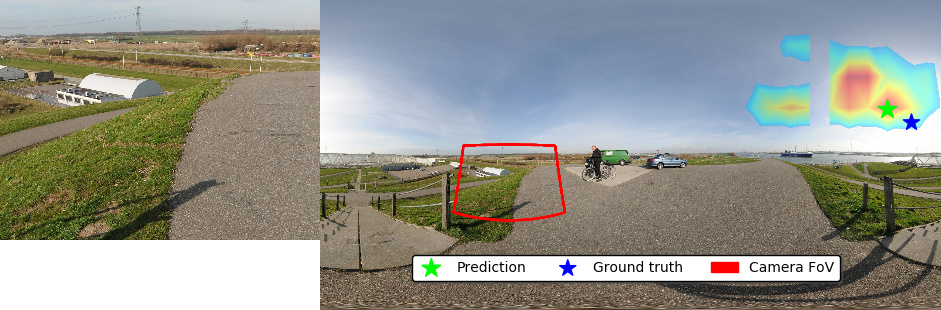
\includegraphics[width=\mywidth]{pano_aaqezlelvvcrrh_005.jpg}\\
Angular distance: 15.0 degrees

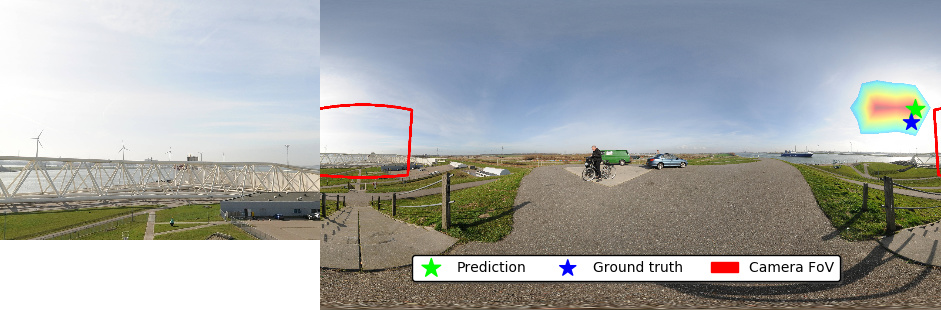
\includegraphics[width=\mywidth]{pano_aaqezlelvvcrrh_002.jpg}\\
Angular distance: 7.8 degrees

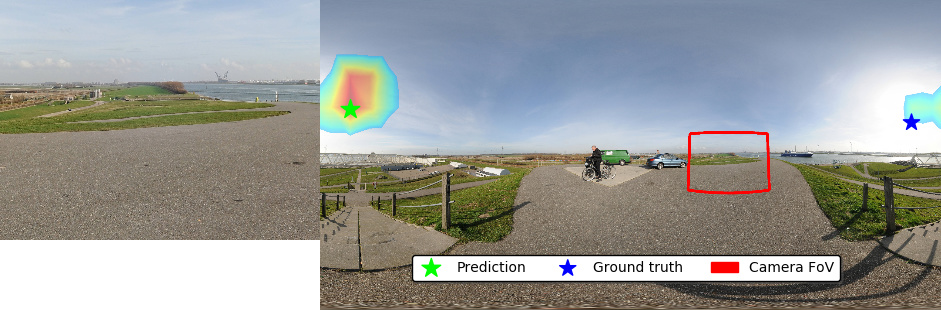
\includegraphics[width=\mywidth]{pano_aaqezlelvvcrrh_006.jpg}\\
Angular distance: 32.3 degrees

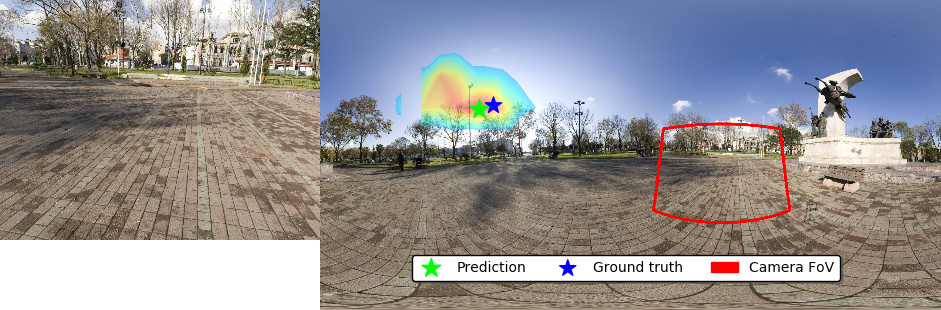
\includegraphics[width=\mywidth]{pano_aaqhsrljfiqght_005.jpg}\\
Angular distance: 7.4 degrees

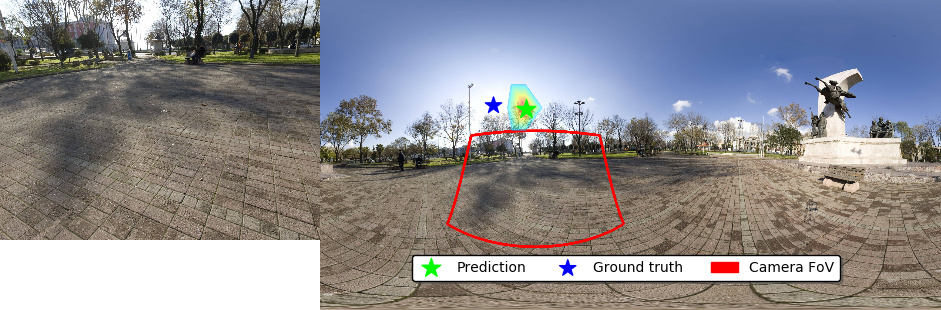
\includegraphics[width=\mywidth]{pano_aaqhsrljfiqght_002.jpg}\\
Angular distance: 16.8 degrees

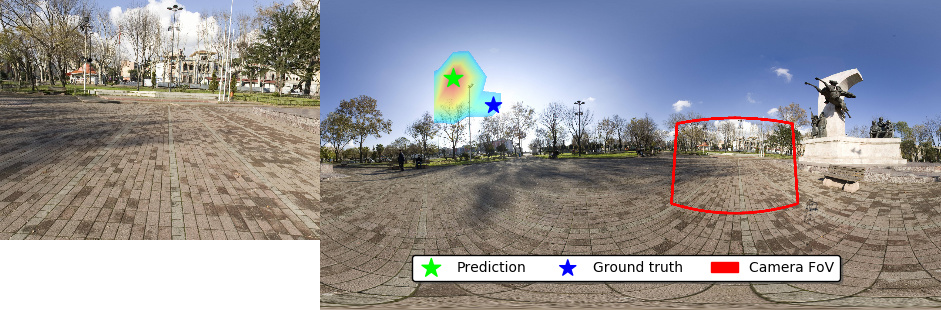
\includegraphics[width=\mywidth]{pano_aaqhsrljfiqght_003.jpg}\\
Angular distance: 24.1 degrees

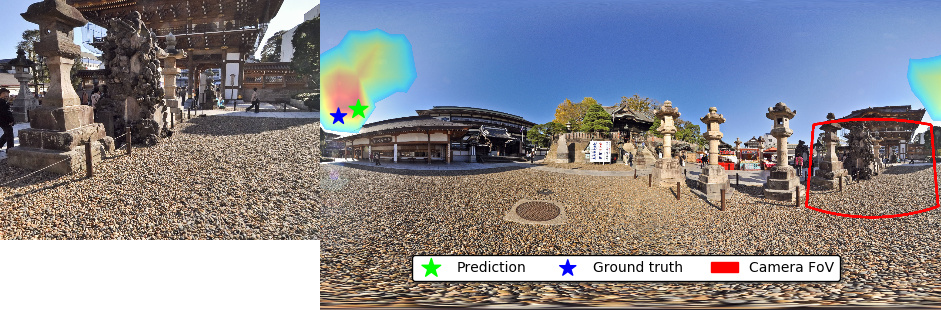
\includegraphics[width=\mywidth]{pano_aaqpmaoqocdqfu_007.jpg}\\
Angular distance: 11.3 degrees

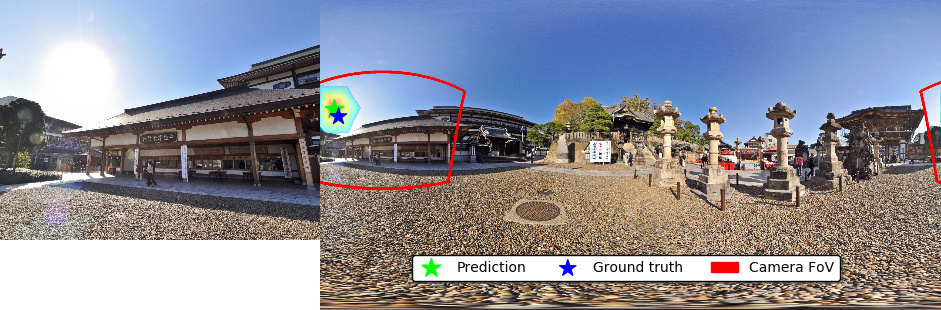
\includegraphics[width=\mywidth]{pano_aaqpmaoqocdqfu_006.jpg}\\
Angular distance: 4.7 degrees

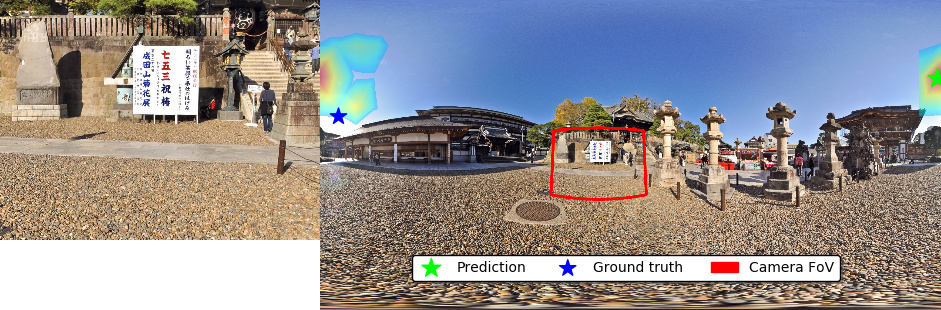
\includegraphics[width=\mywidth]{pano_aaqpmaoqocdqfu.jpg}\\
Angular distance: 24.2 degrees

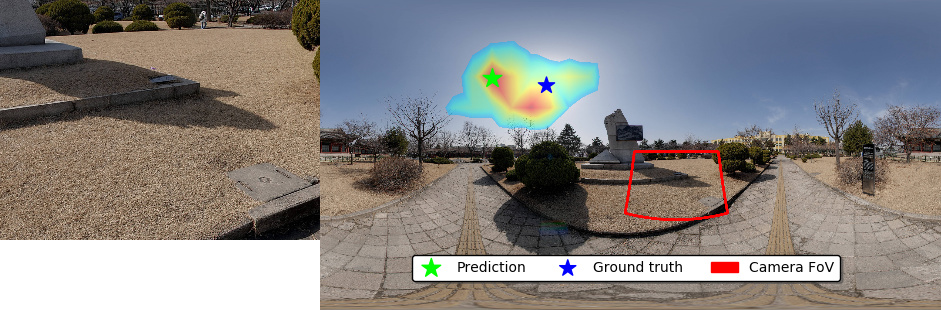
\includegraphics[width=\mywidth]{pano_aarqodbwuocbxc_005.jpg}\\
Angular distance: 23.3 degrees

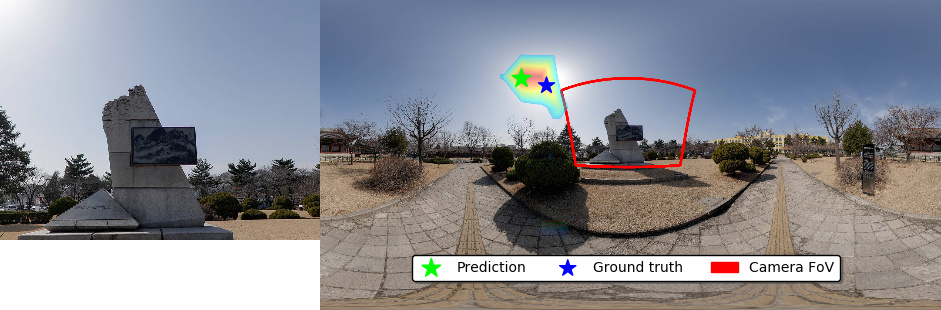
\includegraphics[width=\mywidth]{pano_aarqodbwuocbxc_003.jpg}\\
Angular distance: 11.4 degrees

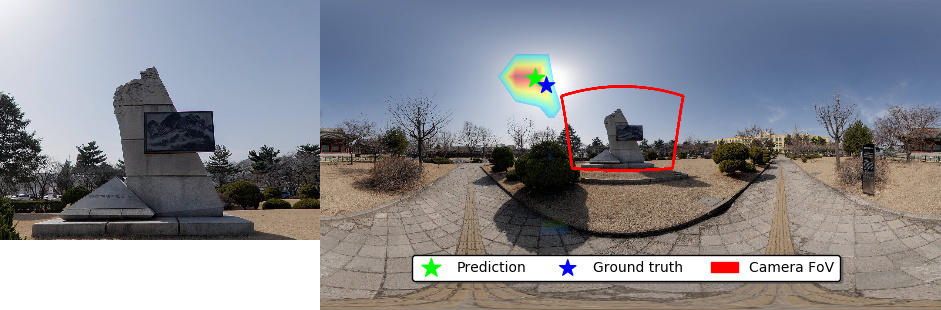
\includegraphics[width=\mywidth]{pano_aarqodbwuocbxc.jpg}\\
Angular distance: 6.2 degrees

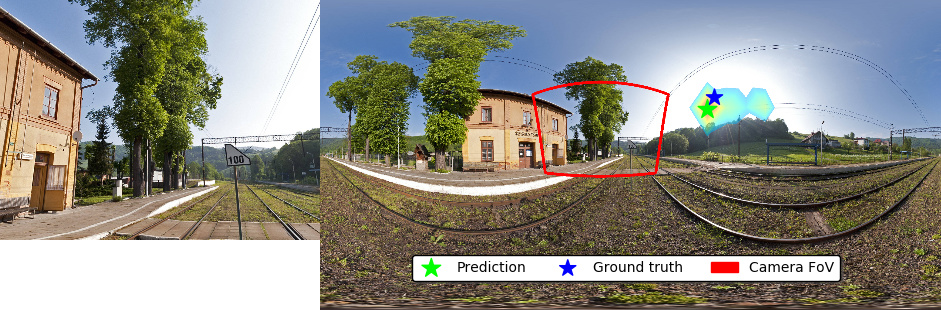
\includegraphics[width=\mywidth]{pano_aasclkvkavzoym_003.jpg}\\
Angular distance: 7.6 degrees

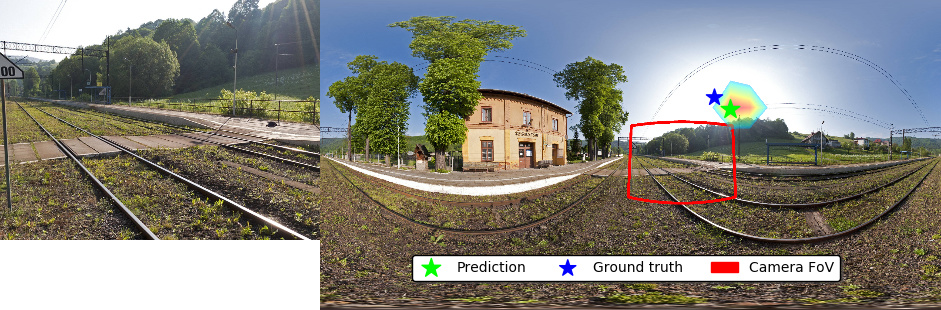
\includegraphics[width=\mywidth]{pano_aasclkvkavzoym_005.jpg}\\
Angular distance: 10.6 degrees

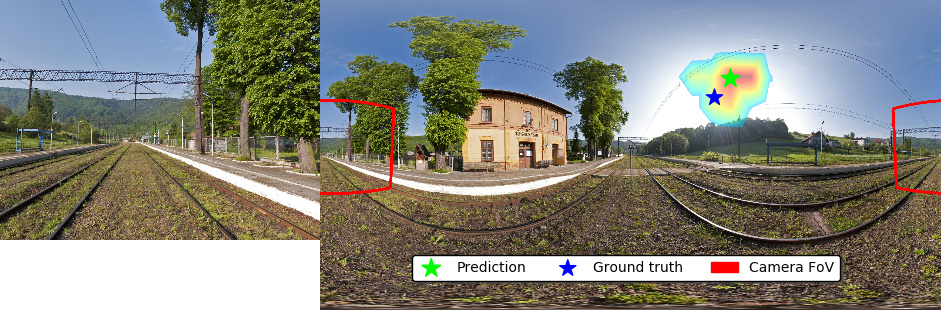
\includegraphics[width=\mywidth]{pano_aasclkvkavzoym_006.jpg}\\
Angular distance: 13.5 degrees

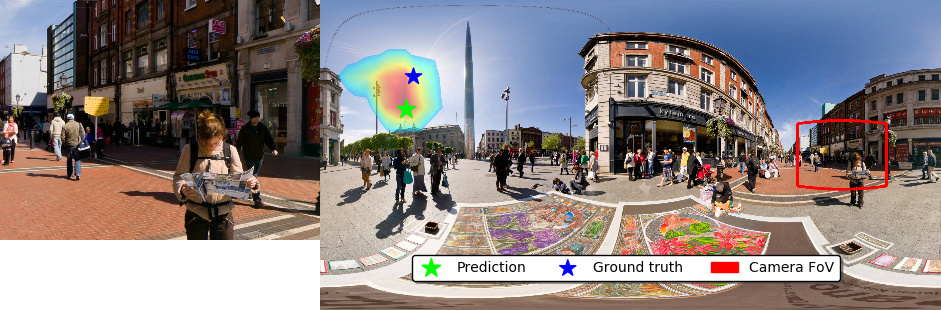
\includegraphics[width=\mywidth]{pano_aasokgzjhapcau_002.jpg}\\
Angular distance: 19.5 degrees

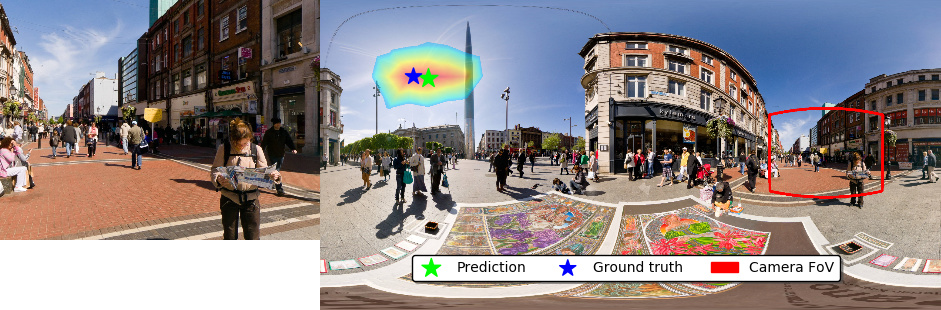
\includegraphics[width=\mywidth]{pano_aasokgzjhapcau_003.jpg}\\
Angular distance: 6.5 degrees

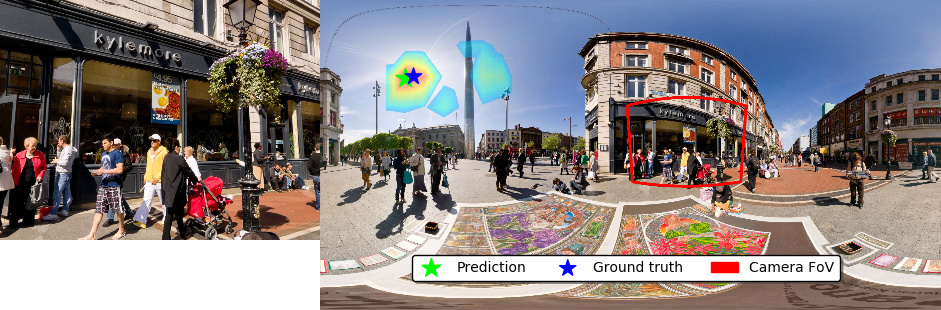
\includegraphics[width=\mywidth]{pano_aasokgzjhapcau_004.jpg}\\
Angular distance: 3.3 degrees

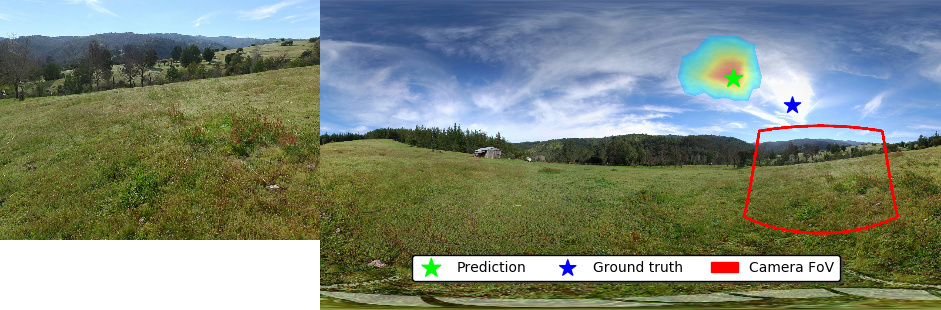
\includegraphics[width=\mywidth]{pano_aaxximpglpmmvj_005.jpg}\\
Angular distance: 31.3 degrees

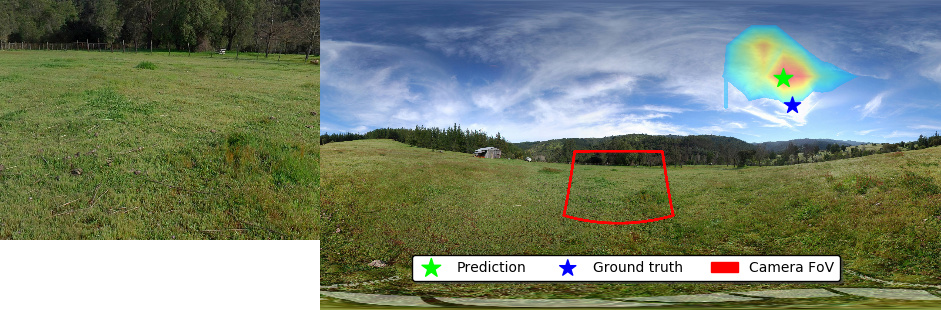
\includegraphics[width=\mywidth]{pano_aaxximpglpmmvj_002.jpg}\\
Angular distance: 16.5 degrees

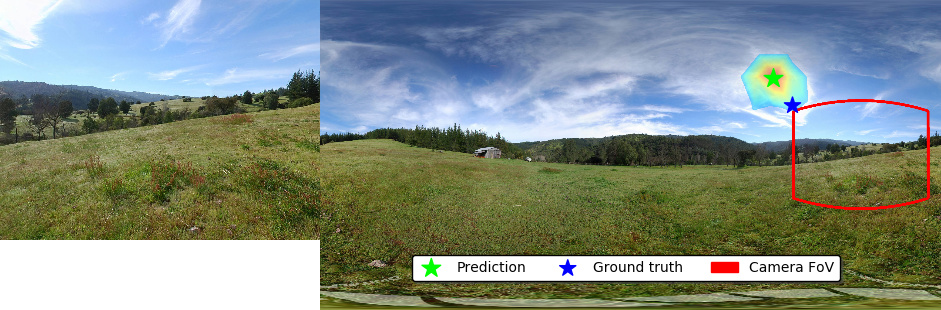
\includegraphics[width=\mywidth]{pano_aaxximpglpmmvj_004.jpg}\\
Angular distance: 18.2 degrees

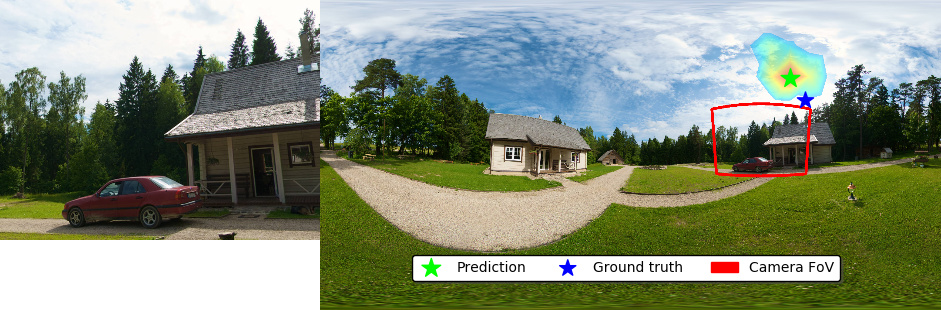
\includegraphics[width=\mywidth]{pano_aazdyyemiqnyfe_005.jpg}\\
Angular distance: 14.4 degrees

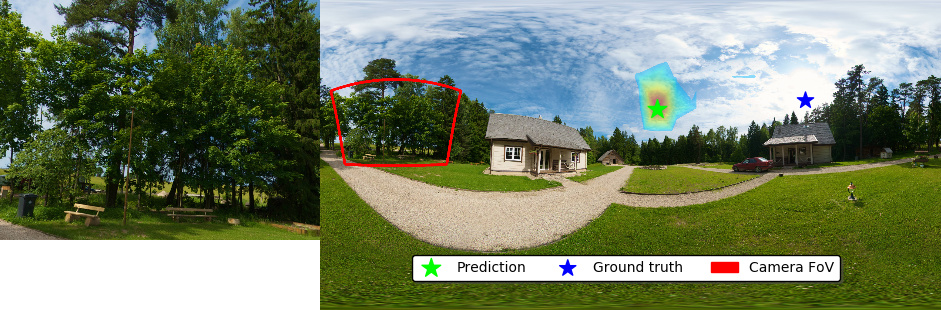
\includegraphics[width=\mywidth]{pano_aazdyyemiqnyfe.jpg}\\
Angular distance: 72.5 degrees

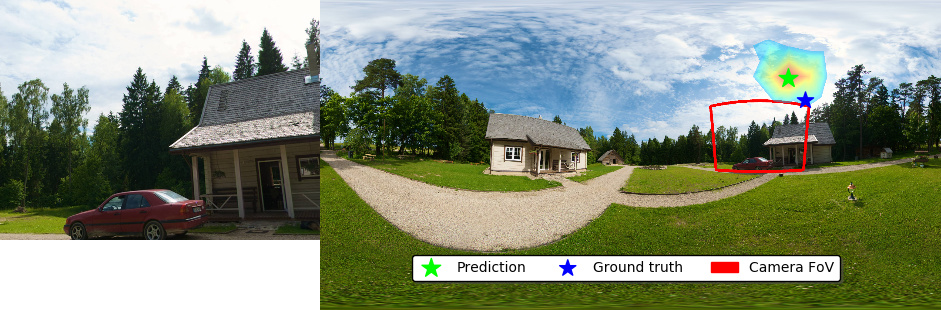
\includegraphics[width=\mywidth]{pano_aazdyyemiqnyfe_002.jpg}\\
Angular distance: 14.7 degrees

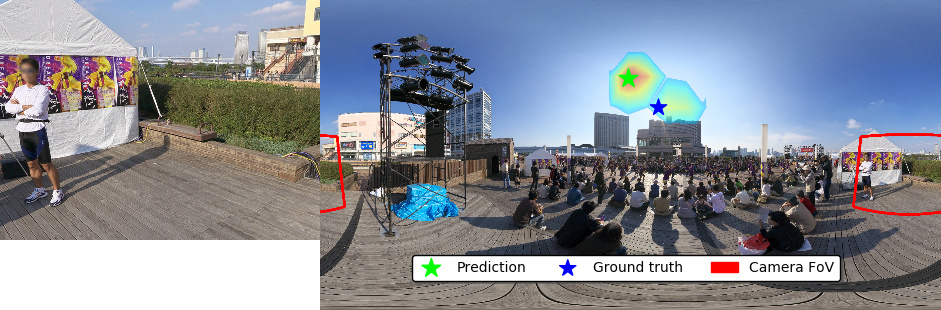
\includegraphics[width=\mywidth]{pano_abapzyetpqwuls_002.jpg}\\
Angular distance: 21.8 degrees

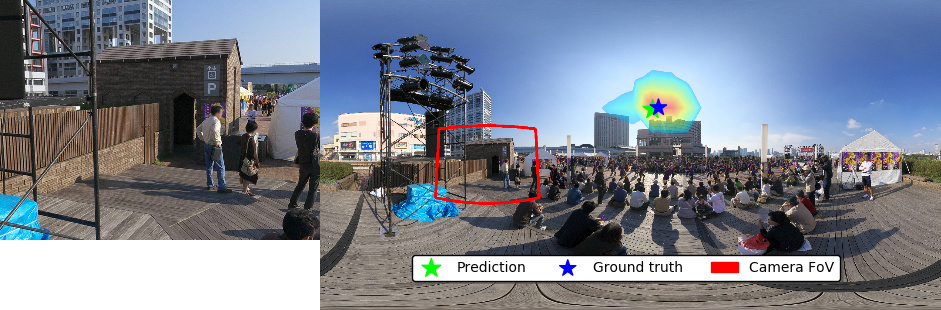
\includegraphics[width=\mywidth]{pano_abapzyetpqwuls_003.jpg}\\
Angular distance: 3.1 degrees

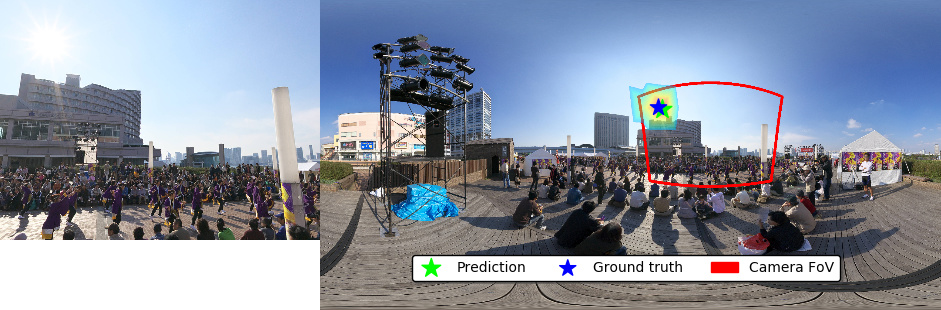
\includegraphics[width=\mywidth]{pano_abapzyetpqwuls_006.jpg}\\
Angular distance: 2.3 degrees

\end{multicols}

\protect\hypertarget{virtualobjectinsert}{}{}

\hypertarget{virtual-object-insertion}{%
\section{Virtual object
insertion}\label{virtual-object-insertion}}

More virtual object insertion results on the SUN360 dataset are
presented in this section, extending the results of fig. 9. For these
examples, the virtual camera parameters are kept at a fixed value
(fov=60 degrees, elevation=0 degrees). Please see
\protect\hyperlink{camparaminsertionex}{this section} for examples where
camera parameters are set by our CNN.

\begin{multicols}{3}

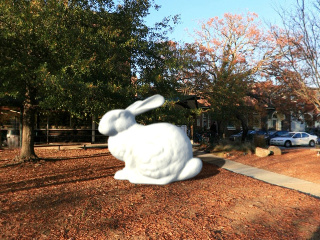
\includegraphics[width=\mywidth]{pano_amclvftibwceyr.jpg}

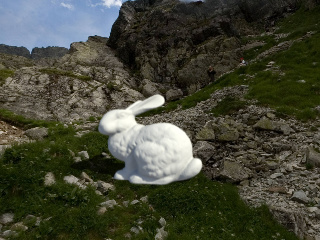
\includegraphics[width=\mywidth]{pano_aoexvqbqucbcuw.jpg}

\includegraphics[width=\mywidth]{pano_apkqohzzaljfyl.jpg}

\includegraphics[width=\mywidth]{pano_aqamdutlzvraki.jpg}

\includegraphics[width=\mywidth]{pano_amshyzgawxszwy.jpg}

\includegraphics[width=\mywidth]{pano_aojrzforebnjfs.jpg}

\includegraphics[width=\mywidth]{pano_apraeyhpkndfbl.jpg}

\includegraphics[width=\mywidth]{pano_aqfnsmhtrqbblm.jpg}

\includegraphics[width=\mywidth]{pano_anfgcccjlbzzhv.jpg}

\includegraphics[width=\mywidth]{pano_aotlotniqjfhrm.jpg}

\includegraphics[width=\mywidth]{pano_aptzailmnatdvm.jpg}

\includegraphics[width=\mywidth]{pano_aqiyqsmecvspfu.jpg}

\end{multicols}

\protect\hypertarget{camparameval}{}{}

\hypertarget{camera-parameters-evaluation}{%
\section{Camera parameters
evaluation}\label{camera-parameters-evaluation}}

\protect\hypertarget{camparamestimperf}{}{}

\hypertarget{parameter-estimation-performance}{%
\subparagraph{3.1 Parameter estimation
performance}\label{parameter-estimation-performance}}

In this section, we show a quantitative evaluation of the neural network
estimation performance on the camera elevation (a)-(b) and the camera
field of view (c)-(d). The range of camera elevation in our dataset is
{[}-20, 20{]} degrees, with a absolute median of 10 degrees, as shown in
the blue bar of the cumulative distribution function (a). Note that
estimating camera elevation is analogous to finding the horizon. Our
method recovers a camera elevation within 5 degrees of error roughly
75\% of the time. The camera field of view is measured vertically and
has a range of {[}35, 68{]} degrees in our dataset, with a median of 52
degrees. The proposed method recovers the vertical field of view within
10 degrees roughly 75\% of the time. The distributions of errors on
(b)-(d) are displayed as box-percentile plots, where the envelope width
represents the percentile. The width is maximal at the median (also
shown using a red bar), half the size at the 25th and 75th percentile,
etc.

\begin{tabular}{@{}cc@{}}
\includegraphics[width=0.45\linewidth]{cdf_2.png} &
\includegraphics[width=0.45\linewidth]{cdf_3.png} \\
\small \shortstack{(a) Cumulative distribution function\\ on the camera elevation.} & \small \shortstack{(b) Cumulative distribution function\\ on the camera field of view.} \\
\includegraphics[width=0.45\linewidth]{box-percentile_plot_2.png} &
\includegraphics[width=0.45\linewidth]{box-percentile_plot_3.png} \\
\small (c) Box-Percentile plot on the camera elevation. & \small \shortstack{(d) Box-Percentile plot on\\ the camera field of view.} \\
\end{tabular}

\protect\hypertarget{camparaminsertionex}{}{}

\hypertarget{object-insertion-examples}{%
\subparagraph{3.2 Object insertion
examples}\label{object-insertion-examples}}

\subsection{Camera Elevation}

For the following results, we allow the neural network to control the
elevation angle (up-down axis) of the camera while performing a virtual
object insertion. The camera's field of view was fixed to 60 degrees for
those experiments.

\begin{multicols}{2}

\begin{minipage}{\linewidth}
\includegraphics[width=\mywidth]{pano_aaqpmaoqocdqfu_005.jpg}\\
Est. elevation: -16 degrees\\
Real elevation: -19 degrees\\
\end{minipage} \\
~\\
\begin{minipage}{\linewidth}
\includegraphics[width=\mywidth]{pano_aczfirgbavyyri_002.jpg}\\
Est. elevation: -6 degrees\\
Real elevation: -11 degrees\\
\end{minipage} \\
~\\
\begin{minipage}{\linewidth}
\includegraphics[width=\mywidth]{pano_aaqpmaoqocdqfu_002.jpg}\\
Est. elevation: -3 degrees\\
Real elevation: 0 degrees\\
\end{minipage} \\
~\\
\begin{minipage}{\linewidth}
\includegraphics[width=\mywidth]{pano_aczfirgbavyyri.jpg}\\
Est. elevation: -13 degrees\\
Real elevation: -17 degrees\\
\end{minipage} \\

\end{multicols}

\subsection{Camera Elevation and Field of View}

We now present examples of virtual object insertion where the neural
network has control over both the camera's elevation angle and field of
view.

\begin{multicols}{2}

\includegraphics[width=\mywidth]{pano_aizkyyutyizoaz.jpg}\\
\small Est. elevation: -18 degrees, FoV: 41 degrees\\
\small Real elevation: -16 degrees, FoV: 40 degrees\\
~\\
\includegraphics[width=\mywidth]{pano_ajlwcdjsjcaemh_002.jpg}\\
\small Est. elevation: -16 degrees, FoV: 46 degrees\\
\small Real elevation: -16 degrees, FoV: 45 degrees\\

\includegraphics[width=\mywidth]{pano_aizkyyutyizoaz_002.jpg}\\
\small Est. elevation: -2 degrees, FoV: 52 degrees\\
\small Real elevation: 0 degrees, FoV: 60 degrees\\
~\\
\includegraphics[width=\mywidth]{pano_ajlwcdjsjcaemh.jpg}\\
\small Est. elevation: -2 degrees, FoV: 51 degrees\\
\small Real elevation: -1 degrees, FoV: 59 degrees\\

\end{multicols}

\protect\hypertarget{HDRcaptures}{}{}

\hypertarget{validation-high-dynamic-range}{%
\section{Validation High Dynamic
Range}\label{validation-high-dynamic-range}}

In sec. 6.3, we described the process of HDR panorama capture. An
excerpt of such a capture is shown in this section, displaying the full
dynamic range of a single capture. While most pixels of an outdoor
panorama lie in a relatively limited dynamic range, the pixels
representing the sun require a scale of roughly 1:10,000 to be
unsaturated. Accurately capturing those extremely intense pixels are
mandatory for cast shadows and proper shading to appear in renderings.

\begin{figure}
\centering
\includegraphics[width=\mywidth]{db-sunny.jpg}
\caption{}
\end{figure}

\protect\hypertarget{virtualobjectinsertHDR}{}{}

\hypertarget{virtual-object-insertion-validation-with-hdr-captures}{%
\section{5. Virtual object insertion validation with HDR
captures}\label{virtual-object-insertion-validation-with-hdr-captures}}

In this section we evaluate our CNN by comparing objects rendered under
our estimated lighting (first column) against those rendered with
captured HDR images (left mouse hover and second column), extending the
results of fig. 11. To create these results we capture HDR panoramas
(last column, see Sec 6.3 for details about our HDR capture
methodology), converted them to 8-bit jpegs, sampled limited
field-of-view images from them, and used these images as inputs to our
CNN. As can be seen from these results, our CNN reproduces the ground
lighting conditions faithfully up to a scale factor, and in particular
recovers the direction of the sun accurately (estimated sun direction
also shown on the panoramas). Since our CNN is trained not on HDR data
but on Hosek-Wilkie parameters fit to LDR data, we also evaluate the
error introduced by this step. We do this by fitting the parameters of
the Hošek-Wilkie model to the 8-bit jpeg panoramas and render objects
under this illumination (third column). These results show that part of
the error in lighting estimation (especially in terms of camera
exposure) is caused by the LDR nature of the data.


\def\panoheight{0.25cm}

\begin{minipage}{\linewidth}
\begin{multicols}{4}

Our method\\

\includegraphics[width=\mywidth]{AG8A2749_Panorama_hdr-corrected_003.jpg}

\includegraphics[width=\mywidth]{AG8A2791_Panorama_hdr-corrected_003.jpg}

\includegraphics[width=\mywidth]{AG8A2833_Panorama_hdr-corrected_008.jpg}

\includegraphics[width=\mywidth]{AG8A2833_Panorama_hdr-corrected_005.jpg}

\vfill\null
\columnbreak

Captured lighting\\

\includegraphics[width=\mywidth]{AG8A2749_Panorama_hdr-corrected_002.jpg}

\includegraphics[width=\mywidth]{AG8A2791_Panorama_hdr-corrected.jpg}

\includegraphics[width=\mywidth]{AG8A2833_Panorama_hdr-corrected_003.jpg}

\includegraphics[width=\mywidth]{AG8A2833_Panorama_hdr-corrected_002.jpg}


\vfill\null
\columnbreak

Hošek-Wilkie fit\\

\includegraphics[width=\mywidth]{AG8A2749_Panorama_hdr-corrected_004.jpg}

\includegraphics[width=\mywidth]{AG8A2791_Panorama_hdr-corrected_002.jpg}

\includegraphics[width=\mywidth]{AG8A2833_Panorama_hdr-corrected_006.jpg}

\includegraphics[width=\mywidth]{AG8A2833_Panorama_hdr-corrected_007.jpg}


\vfill\null
\columnbreak

Panorama\\


\includegraphics[width=\mywidth]{AG8A2749_Panorama_hdr-corrected.jpg}\\
\vspace{\panoheight}\\
\includegraphics[width=\mywidth]{AG8A2791_Panorama_hdr-corrected_004.jpg}\\
\vspace{\panoheight}\\
\includegraphics[width=\mywidth]{AG8A2833_Panorama_hdr-corrected.jpg}\\
\vspace{\panoheight}\\
\includegraphics[width=\mywidth]{AG8A2833_Panorama_hdr-corrected_004.jpg}\\

\end{multicols}
\end{minipage}


\begin{minipage}{\linewidth}
\begin{multicols}{4}

Our method\\

\includegraphics[width=\mywidth]{AG8A2875_Panorama_hdr-corrected_012.jpg}

\includegraphics[width=\mywidth]{AG8A2875_Panorama_hdr-corrected_006.jpg}

\includegraphics[width=\mywidth]{AG8A2875_Panorama_hdr-corrected_010.jpg}

\includegraphics[width=\mywidth]{AG8A2917_Panorama_hdr-corrected_008.jpg}

\includegraphics[width=\mywidth]{AG8A2917_Panorama_hdr-corrected_009.jpg}

\includegraphics[width=\mywidth]{AG8A2917_Panorama_hdr-corrected_010.jpg}

\includegraphics[width=\mywidth]{AG8A2917_Panorama_hdr-corrected_012.jpg}

\includegraphics[width=\mywidth]{AG8A2959_Panorama_hdr-corrected_009.jpg}

\includegraphics[width=\mywidth]{AG8A2959_Panorama_hdr-corrected_006.jpg}

% \includegraphics[width=\mywidth]{AG8A2959_Panorama_hdr-corrected_011.jpg}

% \includegraphics[width=\mywidth]{AG8A3001_Panorama_hdr-corrected_004.jpg}

% \includegraphics[width=\mywidth]{AG8A3043_Panorama_hdr-corrected_016.jpg}

% \includegraphics[width=\mywidth]{AG8A3043_Panorama_hdr-corrected_010.jpg}

% \includegraphics[width=\mywidth]{AG8A3043_Panorama_hdr-corrected_004.jpg}

% \includegraphics[width=\mywidth]{AG8A3043_Panorama_hdr-corrected_014.jpg}

% \includegraphics[width=\mywidth]{AG8A3043_Panorama_hdr-corrected_018.jpg}

% \includegraphics[width=\mywidth]{AG8A3085_Panorama_hdr-corrected_003.jpg}

% \includegraphics[width=\mywidth]{AG8A3127_Panorama_hdr-corrected_007.jpg}

% \includegraphics[width=\mywidth]{AG8A3127_Panorama_hdr-corrected_005.jpg}

% \includegraphics[width=\mywidth]{AG8A3169_Panorama_hdr-corrected.jpg}

% \includegraphics[width=\mywidth]{AG8A3602_Panorama_hdr-corrected_003.jpg}



\vfill\null
\columnbreak

Captured lighting\\


\includegraphics[width=\mywidth]{AG8A2875_Panorama_hdr-corrected_011.jpg}

\includegraphics[width=\mywidth]{AG8A2875_Panorama_hdr-corrected_009.jpg}

\includegraphics[width=\mywidth]{AG8A2875_Panorama_hdr-corrected_004.jpg}

\includegraphics[width=\mywidth]{AG8A2917_Panorama_hdr-corrected_007.jpg}

\includegraphics[width=\mywidth]{AG8A2917_Panorama_hdr-corrected_015.jpg}

\includegraphics[width=\mywidth]{AG8A2917_Panorama_hdr-corrected_002.jpg}

\includegraphics[width=\mywidth]{AG8A2917_Panorama_hdr-corrected_004.jpg}

\includegraphics[width=\mywidth]{AG8A2959_Panorama_hdr-corrected_004.jpg}

\includegraphics[width=\mywidth]{AG8A2959_Panorama_hdr-corrected_010.jpg}

% \includegraphics[width=\mywidth]{AG8A2959_Panorama_hdr-corrected_008.jpg}

% \includegraphics[width=\mywidth]{AG8A3001_Panorama_hdr-corrected.jpg}

% \includegraphics[width=\mywidth]{AG8A3043_Panorama_hdr-corrected_015.jpg}

% \includegraphics[width=\mywidth]{AG8A3043_Panorama_hdr-corrected_019.jpg}

% \includegraphics[width=\mywidth]{AG8A3043_Panorama_hdr-corrected_008.jpg}

% \includegraphics[width=\mywidth]{AG8A3043_Panorama_hdr-corrected_013.jpg}

% \includegraphics[width=\mywidth]{AG8A3043_Panorama_hdr-corrected.jpg}

% \includegraphics[width=\mywidth]{AG8A3085_Panorama_hdr-corrected.jpg}

% \includegraphics[width=\mywidth]{AG8A3127_Panorama_hdr-corrected_008.jpg}

% \includegraphics[width=\mywidth]{AG8A3127_Panorama_hdr-corrected_003.jpg}

% \includegraphics[width=\mywidth]{AG8A3169_Panorama_hdr-corrected_004.jpg}

% \includegraphics[width=\mywidth]{AG8A3602_Panorama_hdr-corrected_002.jpg}

\vfill\null
\columnbreak

Hošek-Wilkie fit\\

\includegraphics[width=\mywidth]{AG8A2875_Panorama_hdr-corrected_003.jpg}

\includegraphics[width=\mywidth]{AG8A2875_Panorama_hdr-corrected_005.jpg}

\includegraphics[width=\mywidth]{AG8A2875_Panorama_hdr-corrected.jpg}

\includegraphics[width=\mywidth]{AG8A2917_Panorama_hdr-corrected_011.jpg}

\includegraphics[width=\mywidth]{AG8A2917_Panorama_hdr-corrected_016.jpg}

\includegraphics[width=\mywidth]{AG8A2917_Panorama_hdr-corrected_006.jpg}

\includegraphics[width=\mywidth]{AG8A2917_Panorama_hdr-corrected_014.jpg}

\includegraphics[width=\mywidth]{AG8A2959_Panorama_hdr-corrected_002.jpg}

\includegraphics[width=\mywidth]{AG8A2959_Panorama_hdr-corrected_003.jpg}

% \includegraphics[width=\mywidth]{AG8A2959_Panorama_hdr-corrected_007.jpg}

% \includegraphics[width=\mywidth]{AG8A3001_Panorama_hdr-corrected_003.jpg}

% \includegraphics[width=\mywidth]{AG8A3043_Panorama_hdr-corrected_017.jpg}

% \includegraphics[width=\mywidth]{AG8A3043_Panorama_hdr-corrected_005.jpg}

% \includegraphics[width=\mywidth]{AG8A3043_Panorama_hdr-corrected_012.jpg}

% \includegraphics[width=\mywidth]{AG8A3043_Panorama_hdr-corrected_002.jpg}

% \includegraphics[width=\mywidth]{AG8A3043_Panorama_hdr-corrected_003.jpg}

% \includegraphics[width=\mywidth]{AG8A3085_Panorama_hdr-corrected_004.jpg}

% \includegraphics[width=\mywidth]{AG8A3127_Panorama_hdr-corrected_004.jpg}

% \includegraphics[width=\mywidth]{AG8A3127_Panorama_hdr-corrected_002.jpg}

% \includegraphics[width=\mywidth]{AG8A3169_Panorama_hdr-corrected_002.jpg}

% \includegraphics[width=\mywidth]{AG8A3602_Panorama_hdr-corrected_004.jpg}

\vfill\null
\columnbreak

Panorama\\

\includegraphics[width=\mywidth]{AG8A2875_Panorama_hdr-corrected_002.jpg}\\
\vspace{\panoheight}\\
\includegraphics[width=\mywidth]{AG8A2875_Panorama_hdr-corrected_008.jpg}\\
\vspace{\panoheight}\\
\includegraphics[width=\mywidth]{AG8A2875_Panorama_hdr-corrected_007.jpg}\\
\vspace{\panoheight}\\
\includegraphics[width=\mywidth]{AG8A2917_Panorama_hdr-corrected.jpg}\\
\vspace{\panoheight}\\
\includegraphics[width=\mywidth]{AG8A2917_Panorama_hdr-corrected_003.jpg}\\
\vspace{\panoheight}\\
\includegraphics[width=\mywidth]{AG8A2917_Panorama_hdr-corrected_005.jpg}\\
\vspace{\panoheight}\\
\includegraphics[width=\mywidth]{AG8A2917_Panorama_hdr-corrected_013.jpg}\\
\vspace{\panoheight}\\
\includegraphics[width=\mywidth]{AG8A2959_Panorama_hdr-corrected_012.jpg}\\
\vspace{\panoheight}\\
\includegraphics[width=\mywidth]{AG8A2959_Panorama_hdr-corrected.jpg}

% \includegraphics[width=\mywidth]{AG8A2959_Panorama_hdr-corrected_005.jpg}

% \includegraphics[width=\mywidth]{AG8A3001_Panorama_hdr-corrected_002.jpg}

% \includegraphics[width=\mywidth]{AG8A3043_Panorama_hdr-corrected_006.jpg}

% \includegraphics[width=\mywidth]{AG8A3043_Panorama_hdr-corrected_007.jpg}

% \includegraphics[width=\mywidth]{AG8A3043_Panorama_hdr-corrected_011.jpg}

% \includegraphics[width=\mywidth]{AG8A3043_Panorama_hdr-corrected_020.jpg}

% \includegraphics[width=\mywidth]{AG8A3043_Panorama_hdr-corrected_009.jpg}

% \includegraphics[width=\mywidth]{AG8A3085_Panorama_hdr-corrected_002.jpg}

% \includegraphics[width=\mywidth]{AG8A3127_Panorama_hdr-corrected_006.jpg}

% \includegraphics[width=\mywidth]{AG8A3127_Panorama_hdr-corrected.jpg}

% \includegraphics[width=\mywidth]{AG8A3169_Panorama_hdr-corrected_003.jpg}

% \includegraphics[width=\mywidth]{AG8A3602_Panorama_hdr-corrected.jpg}

\end{multicols}
\end{minipage}